% MCDI501 - Grupo 7 - Formativa 1
% Fuente editable del informe. Los resultados corresponden al análisis F1-1.0.
% Compilador: pdfLaTeX. Ejecutar dos veces para actualizar el índice.
% Los nombres, fecha y datos de portada se editan en el bloque DATOS DEL GRUPO.
% Texto, tablas y ecuaciones son editables directamente en este archivo.
% Las figuras provienen del notebook: actualizar el análisis antes de cambiar cifras.

\documentclass[11pt,a4paper]{article}
\usepackage[utf8]{inputenc}
\usepackage[T1]{fontenc}
% Overleaf y TeX Live completo incluyen el idioma español. En una instalación
% mínima se mantienen las etiquetas españolas sin exigir paquetes adicionales.
\IfFileExists{spanish.ldf}{
  \usepackage[spanish,es-nodecimaldot,es-tabla]{babel}
}{
  \renewcommand{\contentsname}{Índice}
  \renewcommand{\figurename}{Figura}
  \renewcommand{\tablename}{Tabla}
  \renewcommand{\refname}{Referencias}
}
\usepackage{lmodern}
\usepackage[margin=2.5cm]{geometry}
\usepackage{amsmath}
\usepackage{array,tabularx,booktabs}
\usepackage{graphicx,float}
\usepackage{caption}
\usepackage{xcolor,titlesec,fancyhdr}
\usepackage{xurl}
\usepackage{hyperref}
\usepackage{microtype}

\hypersetup{hidelinks,pdftitle={Formativa 1 Exploración e inferencia de lluvias en Australia},
  pdfauthor={Benjamín Araya, Alan Cañete, Patricio Cortez y Jorge Guaico},
  pdfsubject={MCDI501 Estadística Computacional para la Toma de Decisiones}}
\urlstyle{same}
\definecolor{gris}{gray}{0.35}
\titleformat{\section}{\large\bfseries}{\thesection.}{0.5em}{}
\titleformat{\subsection}{\normalsize\bfseries}{\thesubsection}{0.5em}{}
\titlespacing*{\section}{0pt}{0.9em}{0.5em}
\titlespacing*{\subsection}{0pt}{0.8em}{0.35em}
\setlength{\parindent}{0pt}
\setlength{\parskip}{0.45em}
\setlength{\headheight}{14pt}
\setlength{\emergencystretch}{2em}
\setcounter{tocdepth}{1}
\captionsetup{font=small,labelfont=bf,labelsep=period,
  justification=raggedright,singlelinecheck=false,skip=6pt}
\newcolumntype{L}[1]{>{\raggedright\arraybackslash}p{#1}}
\newcolumntype{C}[1]{>{\centering\arraybackslash}p{#1}}
\newcolumntype{Y}{>{\raggedright\arraybackslash}X}

% ===================== DATOS DEL GRUPO =====================
\newcommand{\proyTitulo}{Exploración e inferencia de lluvias en Australia}
\newcommand{\proyIntegrantes}{Benjamín Araya\\Alan Cañete\\Patricio Cortez\\Jorge Guaico}
\newcommand{\proyDataset}{Rain in Australia}
\newcommand{\proyFechaAnalisis}{10 de octubre de 2026}
\newcommand{\proyRepo}{\url{https://github.com/BenjaArayaM/Proyecto-Lluvias-Australia-Grupo7}}

% Rutas relativas: proyecto local, compilación desde la raíz o ZIP para Overleaf.
\graphicspath{{figures/}{../../results/01_formativa1/figures/}{results/01_formativa1/figures/}}
\IfFileExists{logo_unab.png}{\newcommand{\archivoLogo}{logo_unab.png}}
  {\newcommand{\archivoLogo}{reports/01_formativa1/logo_unab.png}}

\pagestyle{fancy}
\fancyhf{}
\fancyhead[L]{\small MCDI501 - Estadística Computacional para la Toma de Decisiones}
\fancyhead[R]{\small Grupo 7}
\fancyfoot[L]{\footnotesize Magíster en Ciencia de Datos e Inteligencia Artificial}
\fancyfoot[R]{\footnotesize Formativa 1 - \thepage}
\renewcommand{\headrulewidth}{0pt}
\renewcommand{\footrulewidth}{0pt}

\begin{document}
% ===================== PORTADA =====================
\thispagestyle{empty}
\begin{center}
\vspace*{0.6cm}
\includegraphics[height=4.0cm]{\archivoLogo}\par
\vspace{1.0cm}
{\large Universidad Andrés Bello\par}
{\normalsize Magíster en Ciencia de Datos e Inteligencia Artificial\par}
\vspace{0.35cm}
{\normalsize MCDI501 - Estadística Computacional para la Toma de Decisiones\par}
\vspace{1.35cm}
{\Large\bfseries Formativa 1\par}
\vspace{0.35cm}
{\LARGE\bfseries \proyTitulo\par}
\vspace{0.65cm}
{\normalsize Informe grupal - Grupo 7 - Ponderación 0\,\%\par}
\vspace{0.8cm}
{\bfseries Integrantes\par}
\vspace{0.2cm}
\begin{tabular}{c}\proyIntegrantes\end{tabular}\par
\vspace{0.65cm}
Dataset: \proyDataset\par
Fecha del análisis: \proyFechaAnalisis\par
\vspace{0.5cm}
{\small Repositorio del grupo\par\proyRepo\par}
\end{center}
\clearpage

% ===================== ALCANCE E ÍNDICE =====================
\section*{Evaluación y alcance}
\textbf{Modalidad:} grupal. \textbf{Evaluación:} Formativa 1, ponderación 0\,\%.
El producto caracteriza el dataset y presenta inferencia exploratoria para decisiones bajo
incertidumbre. Se integra la ficha descriptiva con los criterios estadísticos de la rúbrica.
La entrega se realiza en PDF; la publicación y retroalimentación en el foro de Canvas
son acciones adicionales del grupo. El alcance corresponde a la Fase 1 del enunciado vigente.

\tableofcontents
\clearpage

% ===================== CONTENIDO DEL INFORME =====================

% Introducción
\section{Introducción}

El archivo weatherAUS.csv contiene 145.460 observaciones y 23 variables de 49 localidades entre el 1 de noviembre de 2007 y el 25 de junio de 2017. Entre las etiquetas conocidas, la lluvia al día siguiente aparece en 22,42 \%. La humedad de la tarde presenta una diferencia media de 20,08 puntos porcentuales entre registros con y sin lluvia posterior, al comparar dentro de cada localidad. Este resultado orienta la exploración y conserva límites por dependencia, cobertura desigual y faltantes.


El objetivo de esta formativa es caracterizar el conjunto de datos, reconocer relaciones y aplicar estimación e inferencia básica para fundamentar decisiones bajo incertidumbre. Utilizamos el archivo seleccionado por el grupo y adaptamos los procedimientos docentes a su estructura temporal y geográfica.


\subsection{Ficha del proyecto}

\begin{table}[H]
\centering
\small
\renewcommand{\arraystretch}{1.18}
\setlength{\tabcolsep}{5pt}
\begin{tabularx}{\linewidth}{@{}L{2.7cm}Y@{}}
\toprule

\textbf{Elemento} & \textbf{Descripción} \\
\midrule

Problema & Anticipar la ocurrencia de lluvia al día siguiente a partir de información meteorológica disponible. \\

Unidad observada & Localidad en una fecha. Los registros de una misma localidad se repiten en el tiempo. \\

Objetivo & RainTomorrow, variable cualitativa binaria con valores No y Yes. \\

Aplicación & Orientar planificación agrícola, gestión hídrica y actividades sensibles a la lluvia. \\

Fuente & Rain in Australia, publicación de jsphyg en Kaggle. Datos meteorológicos procedentes del Bureau of Meteorology y procesados en Rattle. \\

Alcance & Exploración, intervalos y prueba t. La evaluación de un modelo predictivo corresponde a fases posteriores. \\

\bottomrule
\end{tabularx}

\end{table}

{\small Repositorio del grupo: \url{https://github.com/BenjaArayaM/Proyecto-Lluvias-Australia-Grupo7}\par}

\clearpage


% Variables y relaciones preliminares
\section{Variables y relaciones preliminares}

Distinguimos el tipo estadístico del tipo de almacenamiento. Una temperatura registrada como número decimal sigue siendo una medida continua; la fecha ordena el panel y las direcciones del viento son categorías con estructura circular. La tabla cubre las 23 columnas originales. El diccionario individual con n observado y faltantes se conserva en el notebook y en diccionario\_variables.csv.


\begin{table}[H]
\centering
\small
\renewcommand{\arraystretch}{1.18}
\setlength{\tabcolsep}{5pt}
\begin{tabularx}{\linewidth}{@{}L{5.7cm}L{6.0cm}Y@{}}
\toprule

\textbf{Variables originales} & \textbf{Tipo estadístico} & \textbf{Unidad} \\
\midrule

Date & Temporal & Fecha \\

Location & Cualitativa nominal & Localidad \\

MinTemp, MaxTemp, Temp9am, Temp3pm & Cuantitativas continuas & \textdegree{}C \\

Rainfall & Cuantitativa continua & mm \\

Evaporation & Cuantitativa continua & mm \\

Sunshine & Cuantitativa continua & Horas \\

WindGustSpeed, WindSpeed9am, WindSpeed3pm & Cuantitativas continuas & km/h \\

WindGustDir, WindDir9am, WindDir3pm & Cualitativas nominales circulares & 16 direcciones \\

Humidity9am, Humidity3pm & Cuantitativas continuas & \% \\

Pressure9am, Pressure3pm & Cuantitativas continuas & hPa \\

Cloud9am, Cloud3pm & Discretas codificadas; orden físico 0 a 8 & Octas; código 9 \\

RainToday, RainTomorrow & Cualitativas nominales binarias & No / Yes \\

\bottomrule
\end{tabularx}

\end{table}

\subsection{Preguntas de investigación}

Examinamos la distribución de lluvia, humedad y temperatura; la diferencia de humedad antes de días con y sin lluvia dentro de la misma localidad; y la variación geográfica y estacional de las frecuencias y de los datos faltantes. Son preguntas exploratorias, sin atribución causal.


La humedad y la nubosidad pueden acompañar condiciones asociadas a lluvia. La precipitación registrada y RainToday permiten estudiar persistencia. Las temperaturas de horarios cercanos pueden compartir información y ocasionar redundancia. Location y Date permiten reconocer que una asociación agrupada mezcla climas, estaciones del año y períodos de observación.


\subsection{Disponibilidad para futuras predicciones}

El diccionario de Rattle ubica la ráfaga máxima en una ventana hasta medianoche y Sunshine resume horas de sol del día (Williams, s. f.). Por ello, los totales y máximos diarios no se consideran automáticamente disponibles al emitir una predicción a las 3 pm. Antes del modelamiento se deberá fijar la hora de emisión y comprobar la disponibilidad de cada predictor. RainTomorrow nunca se utiliza como predictor de sí misma.


\clearpage


% Calidad de datos y variable objetivo
\section{Calidad de datos y variable objetivo}

Se identifican 142.193 etiquetas observadas: No=110.316 y Yes=31.877. Los 3.267 objetivos faltantes representan 2,25 \% del total. Las proporciones por clase utilizan únicamente etiquetas conocidas y no convierten un objetivo ausente en No.


\begin{figure}[H]
\centering
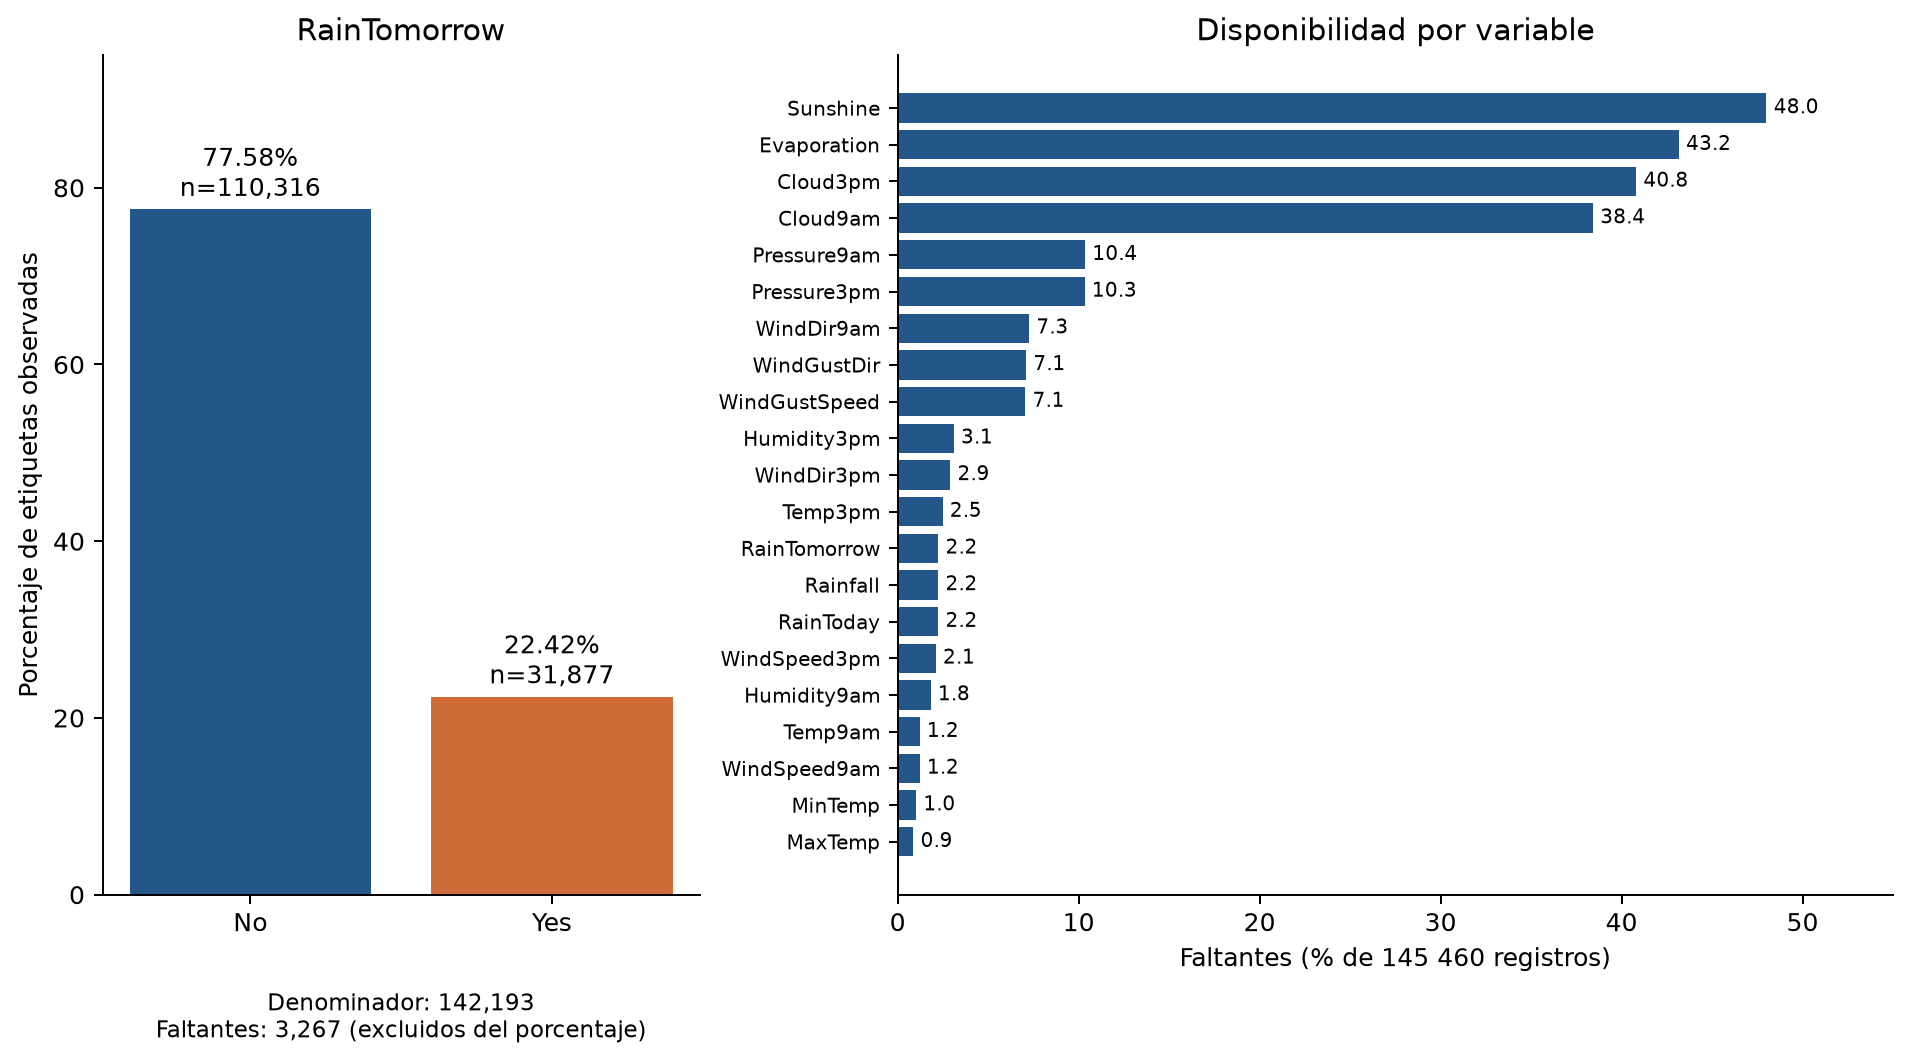
\includegraphics[width=\linewidth,height=8.7cm,keepaspectratio]{01_objetivo_faltantes.png}
\caption{Distribución de RainTomorrow entre 142.193 etiquetas conocidas y porcentaje de faltantes en el archivo completo. Fuente: cálculos propios con el CSV auditado.}
\label{fig:01_objetivo_faltantes}
\end{figure}

No se detectan duplicados exactos ni de localidad y fecha, fechas inválidas, mínima mayor que máxima, humedades fuera de 0 a 100 ni precipitaciones negativas. Sunshine presenta 48,01 \% de faltantes y está ausente en todos los registros de 19 localidades. Evaporation tiene 43,17 \%. Solo 56.420 filas (38,79 \%) son completas en las 23 variables. Se trabaja con exclusiones por cálculo, sin eliminación global.


RainToday coincide con Rainfall > 1 mm en 142.199 pares observados. RainTomorrow coincide con esa regla aplicada al día siguiente en 142.017 pares consecutivos. Esta auditoría no reconstruye etiquetas ni incorpora valores futuros al análisis predictivo. El código 9 aparece dos veces en Cloud9am y una en Cloud3pm. BoM lo documenta como niebla en otro producto (Bureau of Meteorology, 2024, apéndice 2), por lo que se conserva y se revisará su significado histórico.


\clearpage


% Aplicación de estadística descriptiva
\section{Aplicación de estadística descriptiva}

Las estadísticas se calculan sobre los valores observados de cada variable. La desviación estándar (DE) usa n-1 en su denominador. Los mínimos y máximos muestran el rango; cuartiles, IQR, varianza, moda, asimetría y extremos de Tukey están disponibles en descriptivos.csv. No se imputan valores ni se eliminan extremos.


\begin{table}[H]
\centering
\small
\renewcommand{\arraystretch}{1.18}
\setlength{\tabcolsep}{5pt}
\begin{tabularx}{\linewidth}{@{}lrrrrrr@{}}
\toprule

\textbf{Variable} & \textbf{n observado} & \textbf{Media} & \textbf{Mediana} & \textbf{DE} & \textbf{Mínimo} & \textbf{Máximo} \\
\midrule

MinTemp & 143.975 & 12,19 & 12,00 & 6,40 & -8,5 & 33,9 \\

MaxTemp & 144.199 & 23,22 & 22,60 & 7,12 & -4,8 & 48,1 \\

Rainfall & 142.199 & 2,36 & 0,00 & 8,48 & 0,0 & 371,0 \\

Evaporation & 82.670 & 5,47 & 4,80 & 4,19 & 0,0 & 145,0 \\

Sunshine & 75.625 & 7,61 & 8,40 & 3,79 & 0,0 & 14,5 \\

WindGustSpeed & 135.197 & 40,04 & 39,00 & 13,61 & 6,0 & 135,0 \\

WindSpeed9am & 143.693 & 14,04 & 13,00 & 8,92 & 0,0 & 130,0 \\

WindSpeed3pm & 142.398 & 18,66 & 19,00 & 8,81 & 0,0 & 87,0 \\

Humidity9am & 142.806 & 68,88 & 70,00 & 19,03 & 0,0 & 100,0 \\

Humidity3pm & 140.953 & 51,54 & 52,00 & 20,80 & 0,0 & 100,0 \\

Pressure9am & 130.395 & 1.017,65 & 1.017,60 & 7,11 & 980,5 & 1.041,0 \\

Pressure3pm & 130.432 & 1.015,26 & 1.015,20 & 7,04 & 977,1 & 1.039,6 \\

Cloud9am & 89.572 & 4,45 & 5,00 & 2,89 & 0,0 & 9,0 \\

Cloud3pm & 86.102 & 4,51 & 5,00 & 2,72 & 0,0 & 9,0 \\

Temp9am & 143.693 & 16,99 & 16,70 & 6,49 & -7,2 & 40,2 \\

Temp3pm & 141.851 & 21,68 & 21,10 & 6,94 & -5,4 & 46,7 \\

\bottomrule
\end{tabularx}

\caption{Resúmenes de las 16 columnas numéricas. Las unidades se especifican en la ficha de variables. Cloud resume códigos conservados; su máximo 9 no equivale a una cobertura física de nueve octas.}
\label{tab:3}

\end{table}

Rainfall tiene mediana 0,00 mm y media 2,36 mm, con DE 8,48 mm. El predominio de ceros y una cola que alcanza 371,0 mm explican la diferencia entre centro típico y promedio. La regla de Tukey señala 25.578 valores, lo que no implica que sean errores: una distribución asimétrica puede generar muchos señalamientos legítimos.


Humidity3pm tiene mediana 52,00 \%, IQR de 29,00 puntos porcentuales y rango 0 a 100 \%. MaxTemp tiene mediana 22,60 \textdegree{}C y DE 7,12 \textdegree{}C. La variabilidad combina cambios diarios y diferencias geográficas. La moda de medidas continuas depende del redondeo del instrumento y se interpreta junto con mediana y distribución.


\clearpage


% Distribuciones y comparación por clase
\section{Distribuciones y comparación por clase}

\begin{figure}[H]
\centering
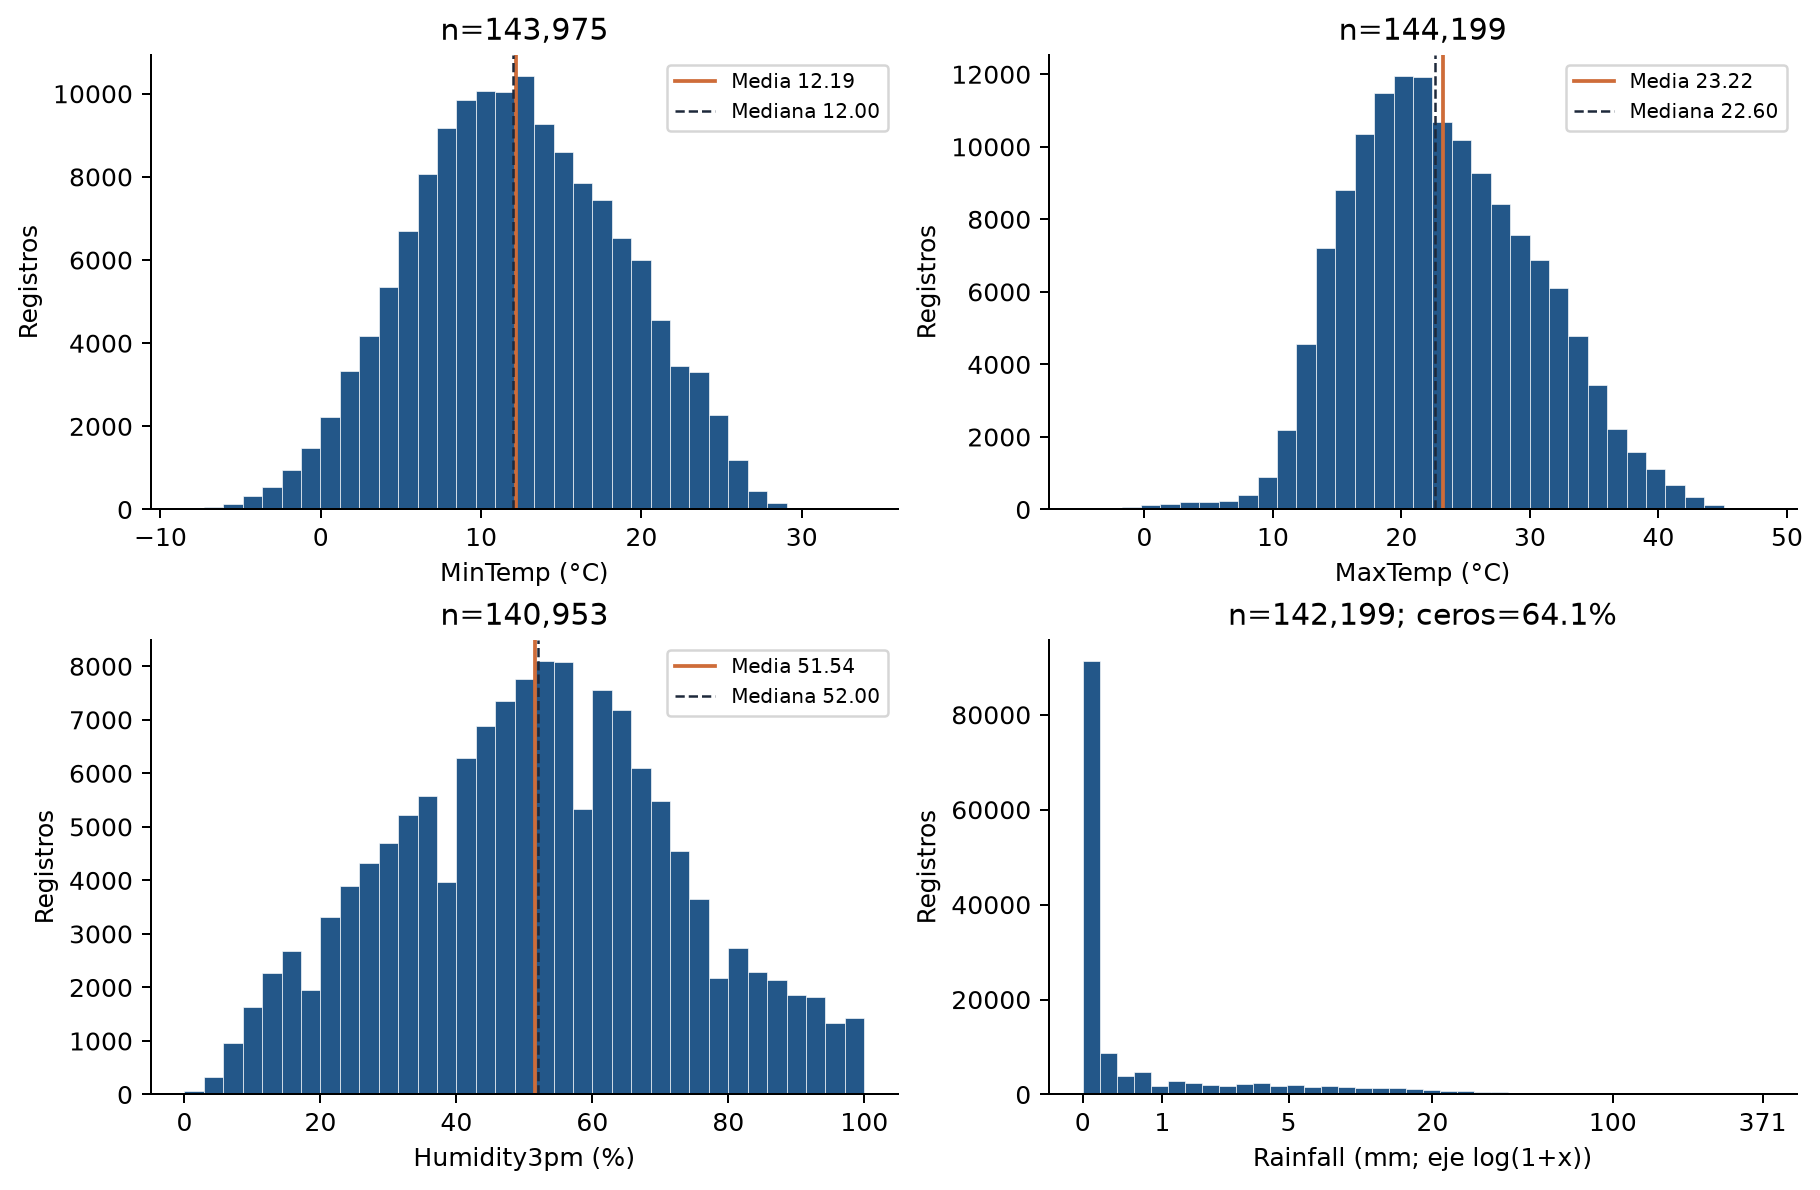
\includegraphics[width=\linewidth,height=7.5cm,keepaspectratio]{02_distribuciones.png}
\caption{Distribuciones de temperatura, humedad y precipitación. Media y mediana corresponden a registros observados. El eje de Rainfall usa log(1+x) para visualizar la cola; el CSV no se transforma.}
\label{fig:02_distribuciones}
\end{figure}

\begin{figure}[H]
\centering
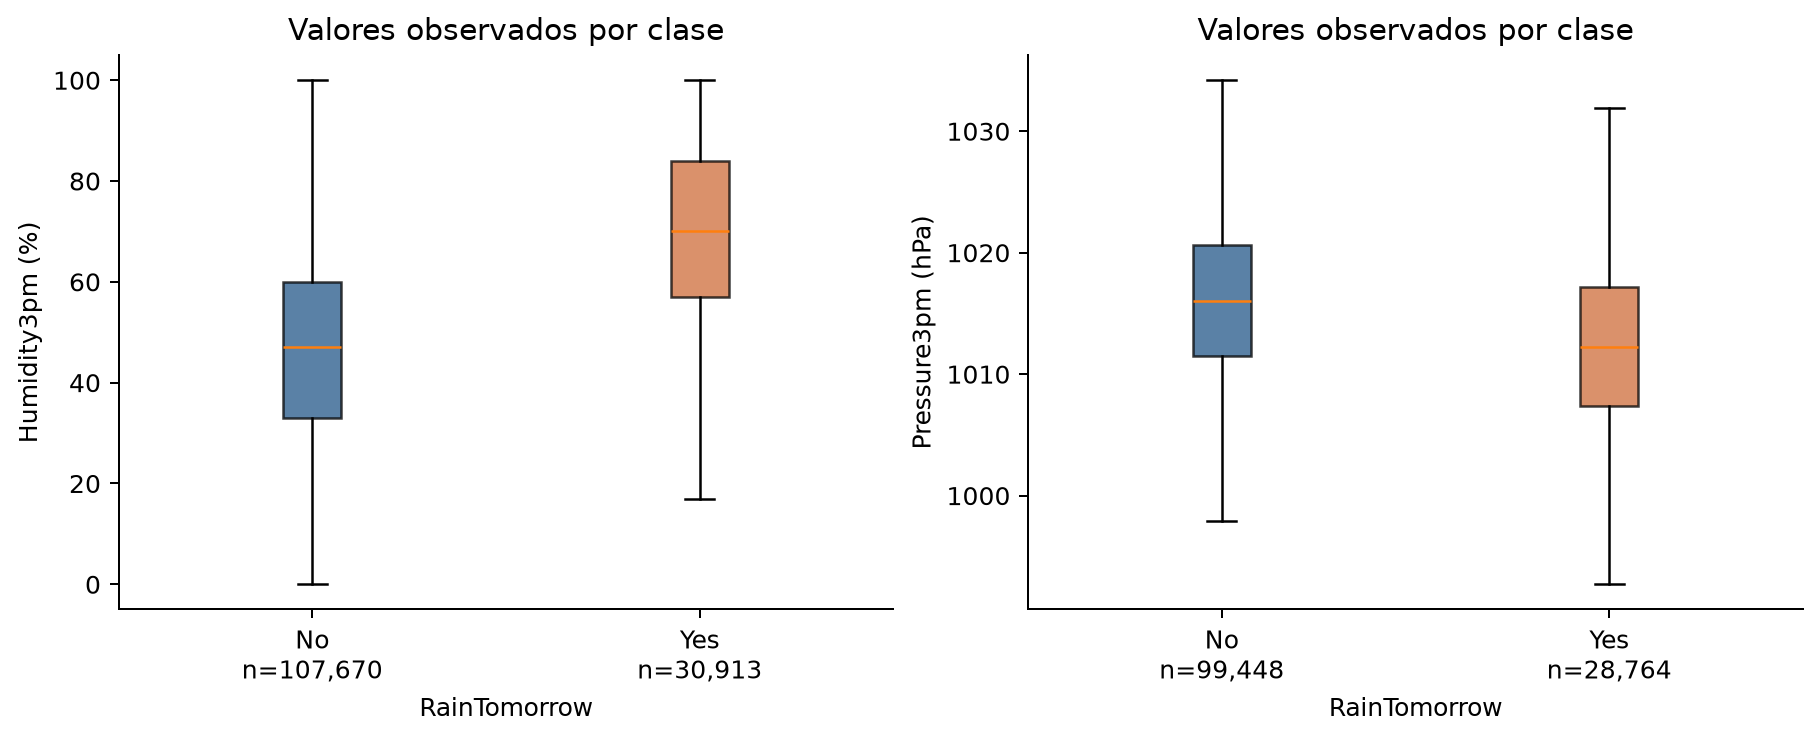
\includegraphics[width=\linewidth,height=8.7cm,keepaspectratio]{03_relaciones_objetivo.png}
\caption{Humedad y presión de la tarde por RainTomorrow. Los puntos exteriores se ocultan solo en el dibujo; todos los datos observados intervienen en los resúmenes. Cada caja informa su n efectivo.}
\label{fig:03_relaciones_objetivo}
\end{figure}

La humedad media agrupada es 46,51 \% para No y 68,80 \% para Yes. La presión media es menor para Yes. El solapamiento entre cajas evidencia incertidumbre individual: una diferencia de medias no constituye una regla de clasificación ni una medida de desempeño.


\clearpage


% Relaciones geográficas y estacionales
\section{Relaciones geográficas y estacionales}

\begin{figure}[H]
\centering
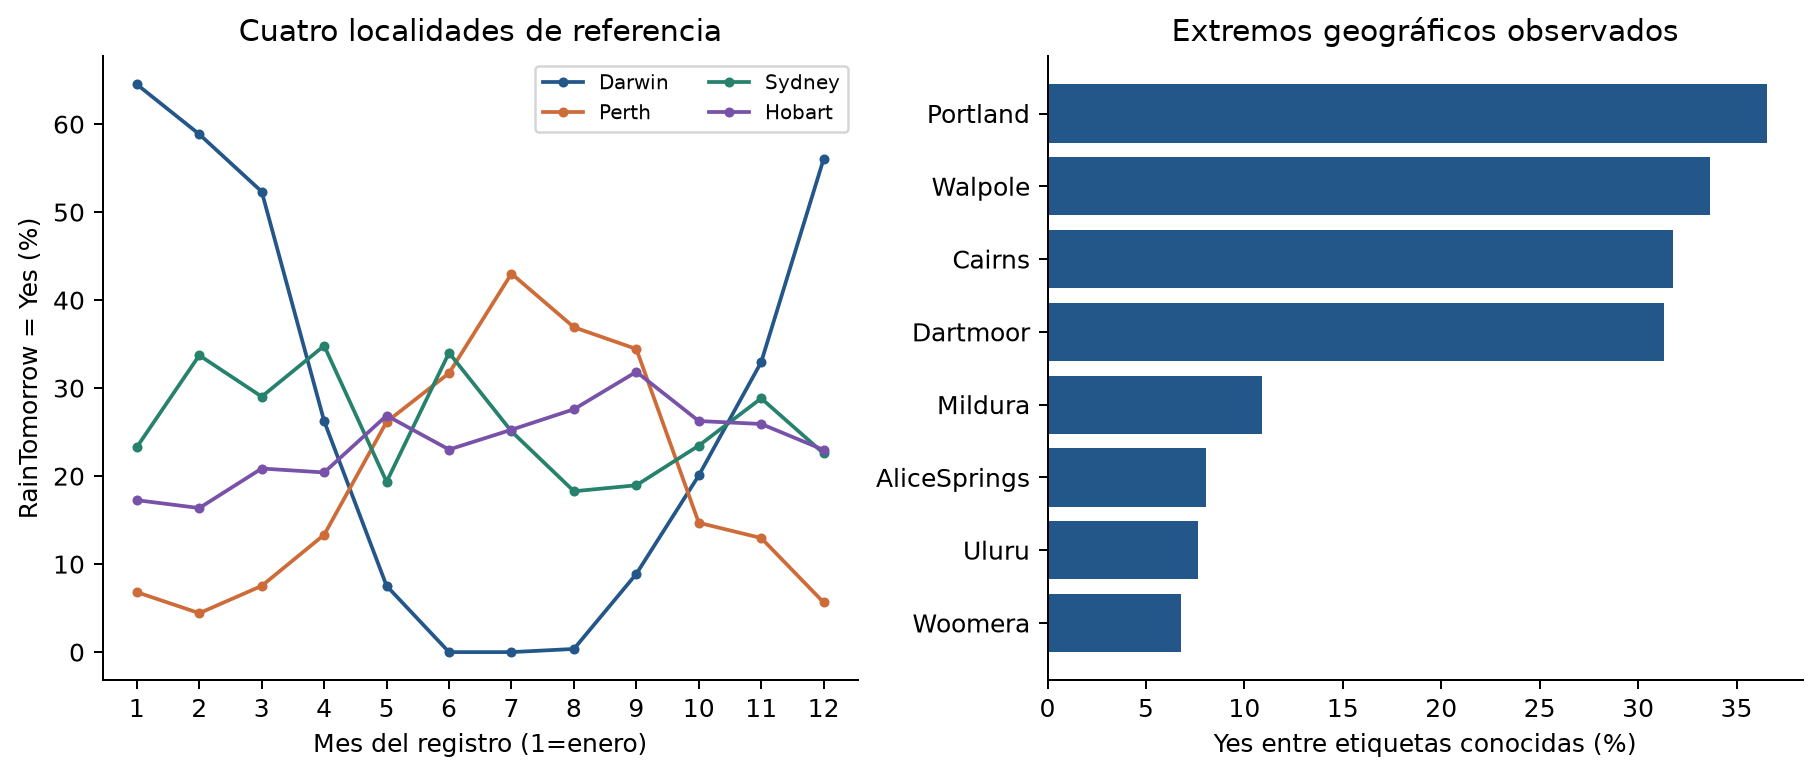
\includegraphics[width=\linewidth,height=8.7cm,keepaspectratio]{05_geografia_estacionalidad.png}
\caption{Frecuencias de Yes por mes del registro en cuatro localidades de referencia y ocho extremos geográficos. Se utilizan etiquetas conocidas; los denominadores y años de cobertura varían.}
\label{fig:05_geografia_estacionalidad}
\end{figure}

El porcentaje de lluvia posterior va de 6,76 \% en Woomera a 36,55 \% en Portland. Darwin presenta mayor frecuencia en meses cálidos y Perth en meses intermedios de su año austral. Estas curvas describen el archivo y no constituyen una climatología nacional equilibrada. Los meses se asignan al registro, sin desplazarlo al día del objetivo.


\begin{table}[H]
\centering
\small
\renewcommand{\arraystretch}{1.18}
\setlength{\tabcolsep}{5pt}
\begin{tabularx}{\linewidth}{@{}Yrr@{}}
\toprule

\textbf{Estación austral} & \textbf{Etiquetas conocidas} & \textbf{Yes (\%)} \\
\midrule

Verano & 34.256 & 20,30 \\

Otoño & 37.397 & 21,89 \\

Invierno & 35.930 & 26,12 \\

Primavera & 34.610 & 21,24 \\

\bottomrule
\end{tabularx}

\caption{Frecuencias agrupadas por estación del año del registro. Las diferencias pueden incluir cambios en composición de localidades y años.}
\label{tab:4}

\end{table}

\begin{table}[H]
\centering
\small
\renewcommand{\arraystretch}{1.18}
\setlength{\tabcolsep}{5pt}
\begin{tabularx}{\linewidth}{@{}Yrr@{}}
\toprule

\textbf{Variable} & \textbf{n pares con objetivo} & \textbf{Spearman con Yes=1} \\
\midrule

Humidity3pm & 138.583 & 0,431 \\

Rainfall & 140.787 & 0,332 \\

Sunshine & 74.377 & -0,438 \\

Pressure3pm & 128.212 & -0,215 \\

MaxTemp & 141.871 & -0,159 \\

\bottomrule
\end{tabularx}

\caption{Asociaciones descriptivas con eliminación por pares. La nubosidad con código 9 se excluye solo de la vista de correlación; se conserva en el archivo original.}
\label{tab:5}

\end{table}

La humedad, precipitación y sol muestran asociaciones de magnitud apreciable con el objetivo, sujetas a muestras distintas. No se calculan p-valores de correlación por fila. La mediana de correlación de humedad entre días exactamente consecutivos por localidad es 0,502, lo que respalda evitar tratar todos los días como réplicas independientes.


\clearpage


% Estimación puntual e intervalos de confianza
\section{Estimación puntual e intervalos de confianza}

Estimamos Humidity3pm, MaxTemp y MinTemp por su importancia meteorológica y cobertura en las 49 localidades. Primero calculamos una media histórica observada por localidad. Luego promediamos esas 49 medias con igual peso. Este estimando corresponde a una localidad con igual probabilidad de selección dentro del conjunto analizado. La media de todas las filas pondera las localidades por sus mediciones y tiene otro significado.


Para las localidades y fechas fijas del CSV, la media es un resumen exacto. La inferencia introduce un modelo de localidades comparables: su parámetro es la media de sus medias históricas observadas. No se dispone de un muestreo probabilístico que permita equipararlo a la media nacional de Australia. Los intervalos se presentan como aproximaciones exploratorias condicionadas a ese modelo.


\[\mathrm{IC}_{95\,\%}=\bar{x}_{L}\pm t_{0{,}975;\,L-1}\frac{s_L}{\sqrt{L}}.\]

Aquí L=49, sL es la desviación entre las medias locales y t es el cuantil de Student con 48 grados de libertad. Cada intervalo se calcula individualmente al 95 \%. No se declara una cobertura conjunta de 95 \% para los tres parámetros.


\begin{table}[H]
\centering
\small
\renewcommand{\arraystretch}{1.18}
\setlength{\tabcolsep}{5pt}
\begin{tabularx}{\linewidth}{@{}Yccc@{}}
\toprule

\textbf{Parámetro} & \textbf{Media local} & \textbf{IC 95 \%} & \textbf{Media por filas} \\
\midrule

Humidity3pm (\%) & 51,25 & 48,02 a 54,47 & 51,54 \\

MaxTemp (\textdegree{}C) & 23,39 & 22,22 a 24,55 & 23,22 \\

MinTemp (\textdegree{}C) & 12,26 & 11,12 a 13,39 & 12,19 \\

\bottomrule
\end{tabularx}

\caption{Estimaciones con igual peso por localidad frente a medias agrupadas. Humedad: 140.953 valores; máxima: 144.199; mínima: 143.975. En los tres cálculos se dispone de 49 medias locales.}
\label{tab:6}

\end{table}

\subsection{Supuestos e interpretación}

La aproximación t requiere localidades aproximadamente independientes y una distribución de sus medias compatible con el procedimiento. Agregar días dentro de una localidad evita la pseudorreplicación diaria, pero no demuestra independencia espacial. Las medias también dependen de los períodos registrados y del mecanismo de observación. Los faltantes podrían sesgar la descripción de las condiciones completas.


Bajo los supuestos, el procedimiento capturaría el parámetro en 95 \% de repeticiones de ese modelo. El intervalo no contiene el 95 \% de los días ni asigna probabilidad 95 \% a un parámetro fijo. La diferencia entre medias locales y medias agrupadas refleja la elección de pesos y debe mantenerse al reutilizar resultados. Shapiro y Q-Q revisan forma de distribución; no validan representatividad ni independencia.


\clearpage


% Aplicación de una prueba de hipótesis
\section{Aplicación de una prueba de hipótesis}

Evaluamos si la humedad de las 3 pm difiere antes de días con y sin lluvia, comparando las dos medias observadas dentro de cada localidad. Para cada localidad, D es la media de Humidity3pm con Yes menos la media con No. El emparejamiento vincula dos medias de una misma localidad; no empareja individualmente días con distinta clase.


\[H_0:\mu_D=0,\qquad H_1:\mu_D\ne0,\qquad\alpha=0{,}05.\]

\[t=\frac{\bar{D}}{s_D/\sqrt{L}},\qquad\mathrm{gl}=L-1.\]

Aplicamos una t de una muestra sobre las 49 diferencias, equivalente a una t pareada de medias locales, con alternativa bilateral. El supuesto de forma se refiere a esas diferencias. No se requiere igualdad de varianzas de los dos conjuntos diarios para esta prueba sobre diferencias (The SciPy community, s. f.-a). La comparación es exploratoria y no ajusta mezcla de meses, años o faltantes.


\begin{table}[H]
\centering
\small
\renewcommand{\arraystretch}{1.18}
\setlength{\tabcolsep}{5pt}
\begin{tabularx}{\linewidth}{@{}Y C{6.5cm}@{}}
\toprule

\textbf{Resultado} & \textbf{Valor} \\
\midrule

Registros con humedad y objetivo & 138.583 \\

Registros excluidos de esta comparación & 6.877 \\

Localidades y grados de libertad & 49 y 48 \\

Diferencia media & 20,08 puntos porcentuales \\

IC 95 \% & 18,47 a 21,68 puntos porcentuales \\

Estadístico t & 25,146 \\

Valor p & \(2{,}747\times10^{-29}\) \\

Diferencias positivas & 49 de 49 localidades \\

Menor n por clase y localidad & No: 618; Yes: 115 \\

\bottomrule
\end{tabularx}

\caption{Comparación principal de humedad con igual peso por localidad. Los conteos y diferencias de todas las localidades se conservan en diferencias\_localidad.csv.}
\label{tab:7}

\end{table}

Bajo independencia aproximada entre localidades, se rechaza H0 a \(\alpha\)=0,05. La magnitud de 20,08 puntos porcentuales respalda investigar Humidity3pm como candidata para anticipar lluvia. No representa un aumento equivalente en la probabilidad de lluvia ni un efecto causal. El valor p mide incompatibilidad con H0 bajo el modelo; no expresa la probabilidad de que H0 sea verdadera. La menor diferencia se observa en Albany (6,57) y la mayor en AliceSprings (33,34), evidenciando heterogeneidad geográfica.


\clearpage


% Diagnóstico y límites de la inferencia
\section{Diagnóstico y límites de la inferencia}

\begin{figure}[H]
\centering
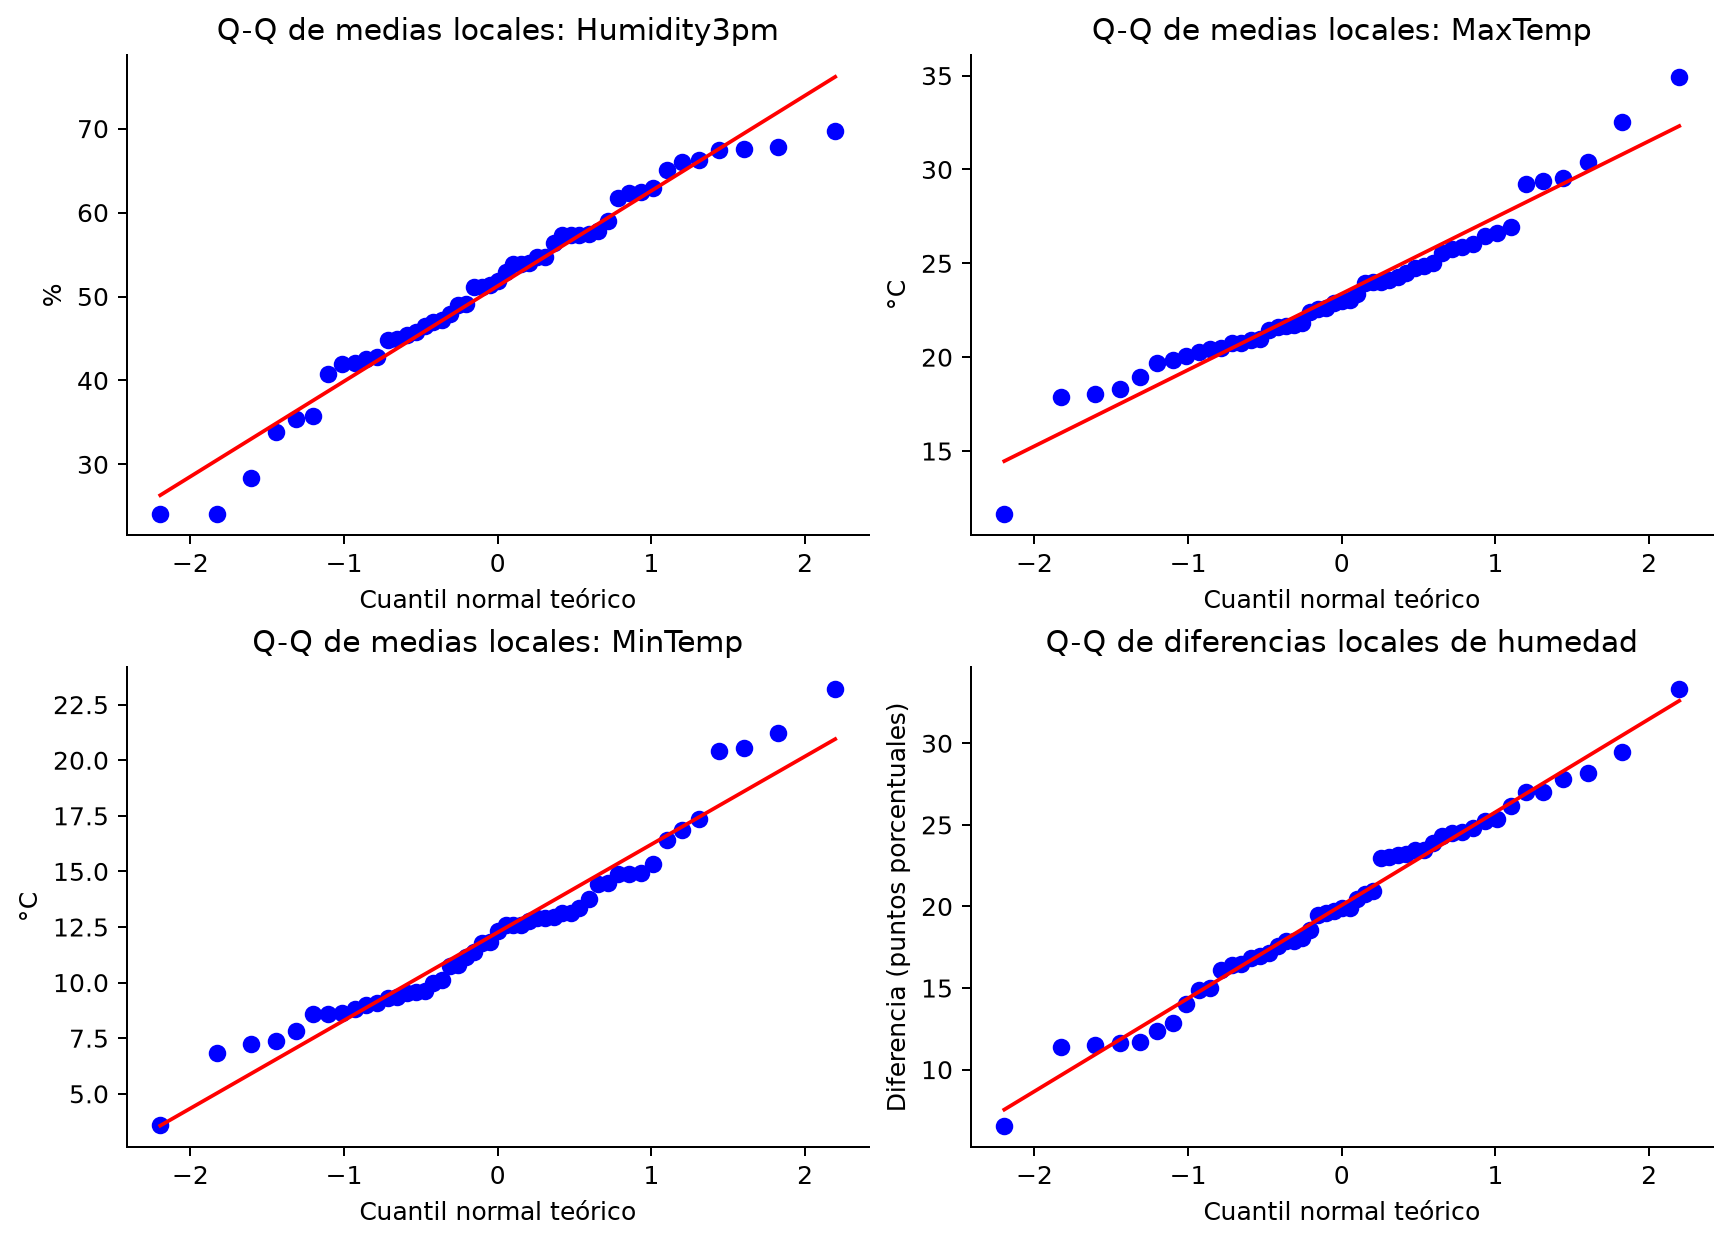
\includegraphics[width=\linewidth,height=8.7cm,keepaspectratio]{06_diagnostico_normalidad.png}
\caption{Gráficos Q-Q de las medias locales de los tres parámetros y de las diferencias locales de humedad. Los desvíos en las colas aconsejan mantener el carácter aproximado de los intervalos.}
\label{fig:06_diagnostico_normalidad}
\end{figure}

\begin{table}[H]
\centering
\small
\renewcommand{\arraystretch}{1.18}
\setlength{\tabcolsep}{5pt}
\begin{tabularx}{\linewidth}{@{}Yrrr@{}}
\toprule

\textbf{Resumen por localidad} & \textbf{Shapiro W} & \textbf{p} & \textbf{Fuera de Tukey} \\
\midrule

Humidity3pm & 0,9654 & 0,1576 & 2 \\

MaxTemp & 0,9642 & 0,1409 & 2 \\

MinTemp & 0,9556 & 0,0623 & 1 \\

Diferencia de Humidity3pm & 0,9884 & 0,9059 & 0 \\

\bottomrule
\end{tabularx}

\caption{Diagnóstico sobre 49 resúmenes, no sobre las filas diarias. Todas las localidades se conservan.}
\label{tab:8}

\end{table}

Shapiro no rechaza normalidad a 0,05 en estos resúmenes; ese resultado no prueba normalidad (The SciPy community, s. f.-b). Los Q-Q muestran desvíos de cola, especialmente en temperaturas. Se mantiene la aproximación t con sus límites. Las diferencias de humedad se alinean mejor y no presentan señalamientos de Tukey. El \(d_z\) entre diferencias locales es 3,592, pero su escala refleja variabilidad entre localidades y no un efecto individual por día.


La principal limitación inferencial es la posible dependencia espacial entre localidades y la cobertura histórica desigual. El archivo no se trata como una muestra aleatoria nacional. La ausencia de mediciones puede depender de estación, período o instrumentación. Ninguno de estos límites queda resuelto por un valor p pequeño. La validación de estabilidad y sensibilidad se conserva como trabajo para la evaluación posterior que corresponda.


\clearpage


% Documentación interpretación y continuidad
\section{Documentación interpretación y continuidad}

\subsection{Procedimiento reproducible}

El notebook 01\_formativa1\_eda\_inferencia.ipynb ejecuta 19 celdas de código desde la raíz encontrada con rutas relativas. Las funciones permanecen en src/formativa1.py. Cada exportación proviene de los valores calculados: 19 tablas CSV, ocho gráficos y resultados.json. El informe se construye a partir de esas exportaciones y conserva los mismos estimandos, unidades y denominadores.


La lectura comprueba 145.460 filas, 23 columnas y el SHA-256 del CSV. Solo se interpreta Date y se crean variables de agrupación en una copia. Los faltantes se excluyen por cálculo con n explícito. Se usa ddof=1, \(\alpha\)=0,05 e IC individuales al 95 \%. La semilla 50107 se registra; esta formativa no realiza remuestreo aleatorio.


Identidad SHA-256 del CSV:\par
{\footnotesize\texttt{573fd715cd69fcacc4df32024d823b450ae3edaae7e8ff2eeb623adbed424014}\par}

La ejecución Work comprobó todas las celdas con ipykernel en memoria. El estudiante acreditó la reproducción completa en JupyterLab Windows mediante su registro del 10 de octubre de 2026. Se conciliaron las 19 tablas y resultados.json; las diferencias numéricas fueron del orden de 1e-14, sin cambiar las cifras publicadas. El CSV permaneció intacto. Las evidencias de ambos entornos se conservan por separado.


\subsection{Interpretación para decisiones bajo incertidumbre}

La humedad de la tarde y la persistencia de lluvia ofrecen relaciones que pueden orientar investigación predictiva. La frecuencia de Yes, cercana a 22,42 \% entre etiquetas conocidas, muestra que los errores de la clase lluvia merecerán atención específica. Una estrategia basada solo en la clase más frecuente puede ocultar fallos relevantes para agricultura o gestión hídrica. Esta formativa no evalúa un clasificador ni determina costos de decisiones.


La disponibilidad de Sunshine y evaporación depende fuertemente de localidad. Una imputación global o una eliminación por casos completos podría alterar la cobertura geográfica. Las decisiones futuras deben considerar ese mecanismo y respetar la separación de entrenamiento y evaluación. No se seleccionan predictores definitivos ni se propone una imputación como resultado de este análisis.


\subsection{Conclusiones}

El conjunto es viable para el proyecto acumulativo por su objetivo binario, sus variables meteorológicas y su cobertura de localidades. La descripción evidencia desbalance, faltantes estructurados y dependencia temporal. La comparación local encuentra humedad mayor antes de días con lluvia en las 49 localidades, con una diferencia promedio de 20,08 puntos porcentuales bajo el estimando definido.


Se conservarán las medias locales de humedad, mínima y máxima, sus conteos, intervalos y diferencias por clase para validar exactamente los mismos parámetros en fases posteriores. El análisis es exploratorio. Las etapas futuras deberán revisar sensibilidad, correlación espacial, mezcla estacional y disponibilidad temporal. Como el archivo completo ya fue explorado, se documentará ese antecedente y todo preprocesamiento del modelo se ajustará dentro del entrenamiento.


\clearpage


% Referencias
\section{Referencias}

Bureau of Meteorology. (2010, 9 de agosto). Definitions for 9am and 3pm statistics. \url{https://www.bom.gov.au/climate/cdo/about/definitions9and3.shtml}


Bureau of Meteorology. (2024, 17 de junio). State-based half hourly observations (72-hour history): User guide (versión 3.2, apéndice 2). \url{https://www.bom.gov.au/catalogue/72_hr_historical_obs.pdf}


jsphyg. (s. f.). Rain in Australia [Conjunto de datos]. Kaggle. \url{https://www.kaggle.com/datasets/jsphyg/weather-dataset-rattle-package/data}


Maidana, J. P. (2026). MCDI501-202682 [Repositorio docente]. \url{https://github.com/jpmaidana/MCDI501-202682}


The SciPy community. (s. f.-a). scipy.stats.ttest\_1samp. \url{https://docs.scipy.org/doc/scipy/reference/generated/scipy.stats.ttest_1samp.html}


The SciPy community. (s. f.-b). scipy.stats.shapiro. \url{https://docs.scipy.org/doc/scipy/reference/generated/scipy.stats.shapiro.html}


Universidad Andrés Bello. (2026). Rúbricas MCDI501 [Archivo Excel, hoja Formativa 1, B3 y filas 42 a 70]. Material proporcionado por el estudiante.


Williams, G. (s. f.). weatherAUS: Daily weather observations from multiple Australian weather stations [Documentación de Rattle]. \url{https://search.r-project.org/CRAN/refmans/rattle/html/weatherAUS.html}


{\small Fuentes web consultadas el 10 de octubre de 2026. La versión histórica del CSV se identifica por su huella; las versiones actuales de Rattle pueden tener dimensiones diferentes.\par}

\subsection{Anexos reproducibles}

El notebook incluye el diccionario de cada columna, todas las frecuencias, los n por pares de correlación, la cobertura de las 49 localidades, tablas de faltantes por localidad y las diferencias individuales usadas por la prueba. Los archivos auxiliares mantienen los datos originales fuera del versionamiento.


\begin{table}[H]
\centering
\small
\renewcommand{\arraystretch}{1.18}
\setlength{\tabcolsep}{5pt}
\begin{tabularx}{\linewidth}{@{}L{9.0cm}Y@{}}
\toprule

\textbf{Ruta dentro del proyecto} & \textbf{Contenido} \\
\midrule

\path{notebooks/01_formativa1_eda_inferencia.ipynb} & Procedimientos ejecutables y salidas \\

\path{results/01_formativa1/tables/} & 19 tablas estadísticas en CSV \\

\path{results/01_formativa1/figures/} & 8 gráficos calculados \\

\path{results/01_formativa1/resultados.json} & Parámetros e identidad del dataset \\

\path{docs/continuidad.md} & Ficha de continuidad \\

\path{evidence/01_formativa1/} & Ejecución y revisión de requisitos \\

\bottomrule
\end{tabularx}

\end{table}

El informe no incluye registros meteorológicos individuales ni adjunta el CSV original. Los anexos permiten verificar los cálculos y conservar evidencia sin duplicar el dataset.


\end{document}
